\chapter{Mesurer le temps}\label{ch:g2:measuring-time}

«~Encore cinq minutes~!~» --- mais combien font-elles, au juste~? Le
temps ne se voit pas, ne se tient pas dans la main, ne se pose pas le
long d'une règle. Et pourtant nous le mesurons tous les jours~: les
courses ont des vainqueurs, les gâteaux sortent du four ni crus ni
brûlés, et l'école finit au bon moment. Voyons comment on apprivoise
le temps.

\section{Instants et durées}

\begin{example}[L'ordre de la journée]\label{ex:g2:measuring-time:order}
Une journée est un défilé d'événements, toujours dans le même ordre~:
le réveil, le petit-déjeuner, l'école, le déjeuner, l'après-midi, le
dîner, le coucher. «~Le petit-déjeuner vient \emph{avant} l'école~»
et «~le dîner vient \emph{après} le déjeuner~» --- avant et après
sont les premiers mots du temps, comme plus long et plus court
étaient les premiers mots de la longueur.
\end{example}

\begin{omfigure}
\begin{tikzpicture}[scale=0.85]
  \draw[-Stealth, very thick] (0,0) -- (11.4,0);
  \foreach \x/\name in {0.8/réveil, 2.9/petit-déjeuner, 5.0/école,
      7.1/déjeuner, 9.2/dîner, 10.7/coucher} {
    \fill[omDef] (\x,0) circle (2.4pt);
    \node[above, font=\small, rotate=40, anchor=south west]
      at (\x,0.15) {\name};
  }
\end{tikzpicture}

{\small Une journée déroulée comme une droite graduée~: chaque
événement a sa place, et la flèche montre dans quel sens le temps
s'écoule --- toujours vers l'avant.}
\end{omfigure}

\begin{definition}[Durée]\label{def:g2:measuring-time:duration}
Un \emph{instant}\index{instant} est un point de la journée~: le
moment où la cloche sonne. Une \emph{durée}\index{durée} est
l'étendue de temps entre deux instants~: de la cloche à la fin de la
leçon. Les instants répondent à la question \emph{quand~?}~; les
durées répondent à \emph{combien de temps~?}
\end{definition}

\begin{example}[Quand, ou combien de
temps~?]\label{ex:g2:measuring-time:whenhowlong}
«~Le film commence après le dîner~» parle d'un instant. «~Le film
dure autant que deux pauses de midi~» parle d'une \omterm{def:g2:measuring-time:duration}{durée}. «~Mon
anniversaire est au printemps~»~: un instant. «~Les vacances ont paru
si courtes~»~: une \omterm{def:g2:measuring-time:duration}{durée} --- et ce chapitre parle surtout de \omterm{def:g2:measuring-time:duration}{durées}.
\end{example}

\section{Comparer des durées}

\begin{method}[Une course honnête entre durées]\label{met:g2:measuring-time:race}
Pour trouver laquelle de deux choses dure le plus longtemps~:
\begin{enumerate}
  \item les faire commencer au \emph{même instant} --- «~à vos
        marques, prêts, partez~!~»~;
  \item regarder laquelle se termine la première~;
  \item celle qui continue quand l'autre est finie dure plus
        longtemps.
\end{enumerate}
Si elles ne peuvent pas se dérouler ensemble (le bain d'aujourd'hui
et le dîner d'hier), fais courir chacune contre une \emph{même}
troisième chose --- un sablier.
\end{method}

\begin{example}[Le sablier]\label{ex:g2:measuring-time:sandtimer}
Un sablier est un petit verre à la taille étranglée~: le sable met
toujours la \emph{même} \omterm{def:g2:measuring-time:duration}{durée} à s'écouler. Cela en fait un arbitre.
Le brossage des dents contre le sablier~: le sable s'est écoulé le
premier --- brosse plus longtemps~! Une chanson contre le sablier~: la
chanson a gagné. La chanson dure donc plus longtemps que le brossage
des dents, alors qu'elles ne se sont jamais affrontées directement.
\end{example}

\begin{omfigure}
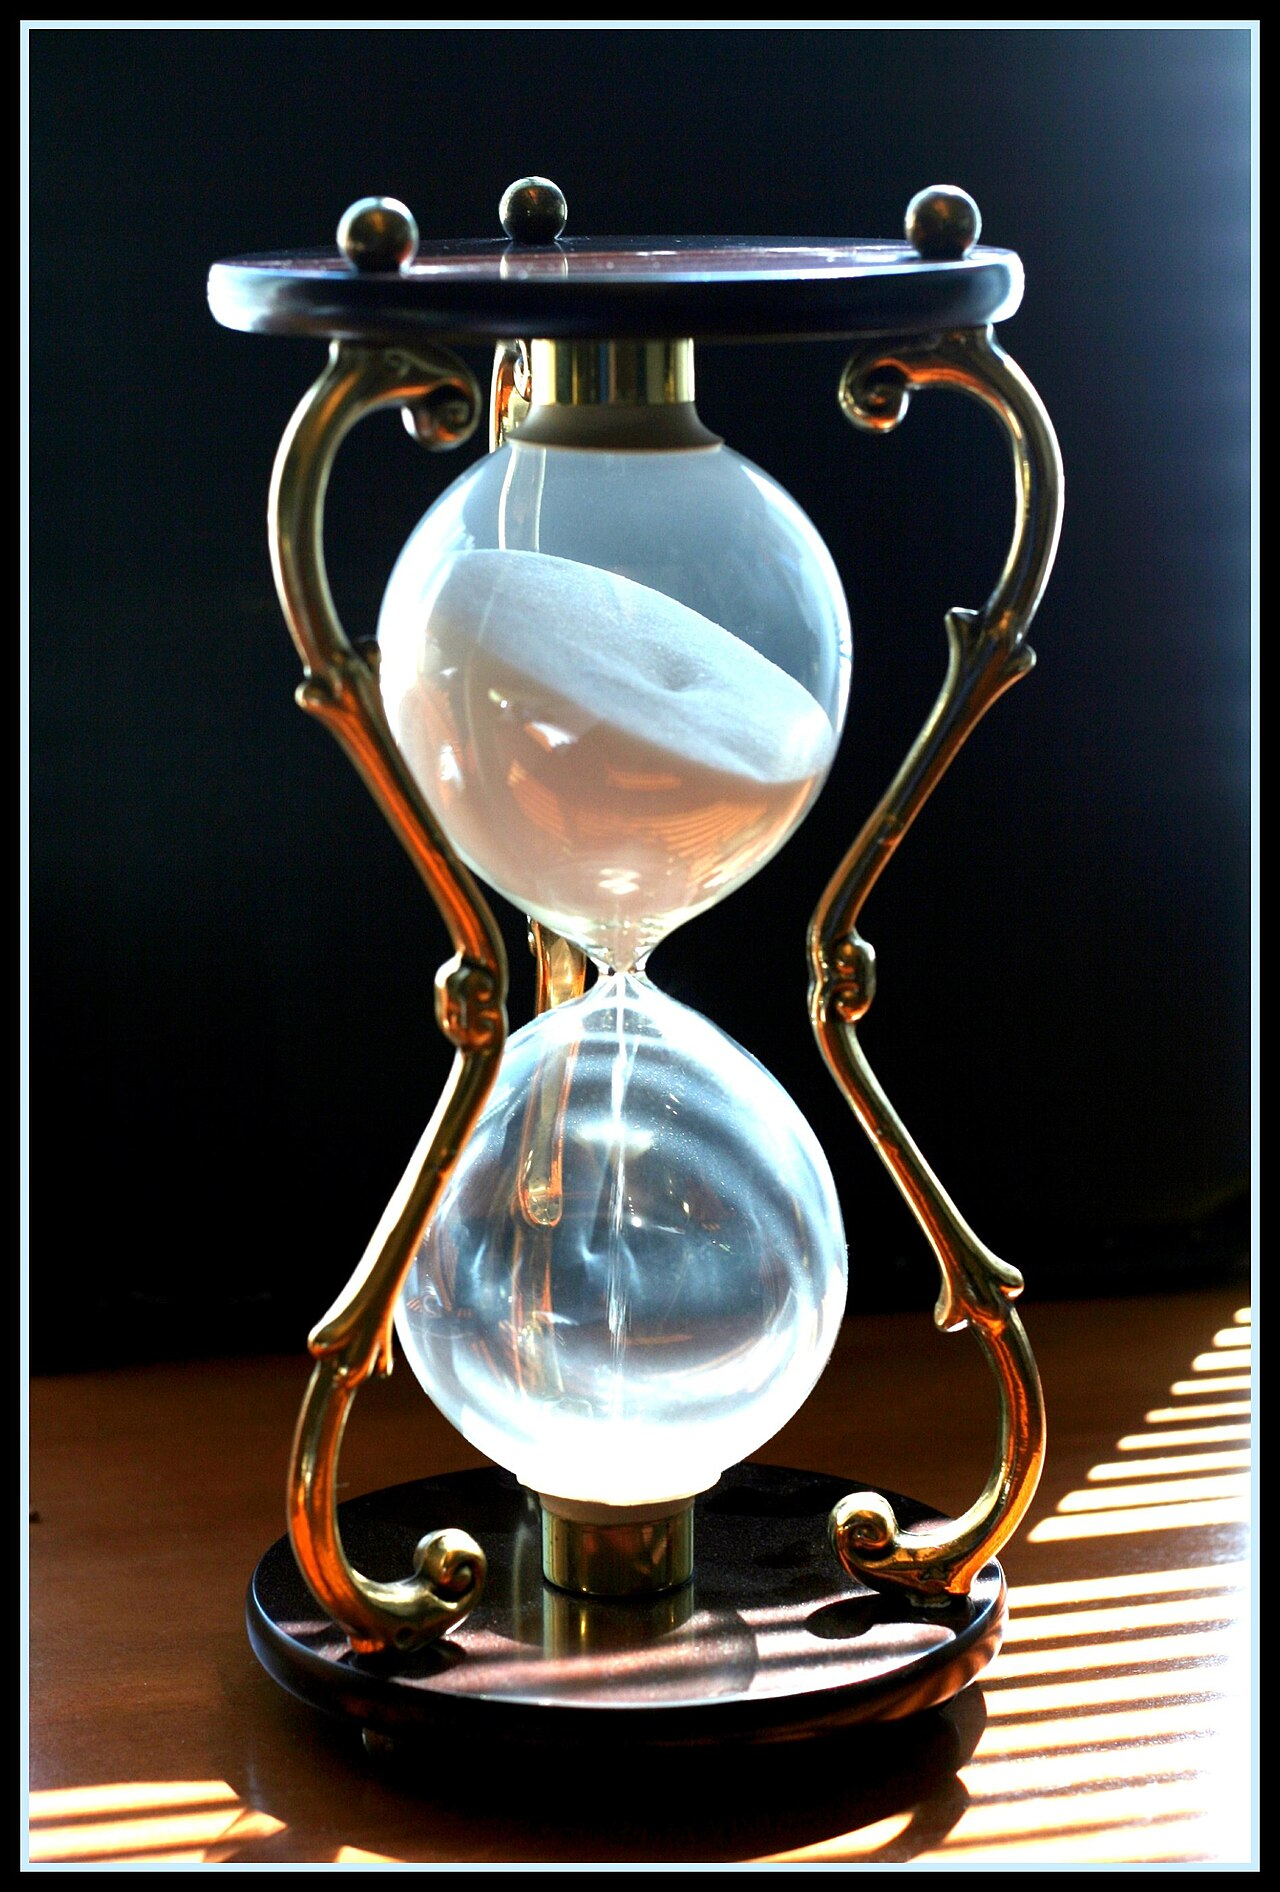
\includegraphics[width=0.34\linewidth]{images/book1/hourglass.jpg}

{\small Un sablier~: une \omterm{def:g2:measuring-time:duration}{durée} que l'on peut tenir dans la main. Le
sable met toujours le même temps à se faufiler par la taille
étranglée --- retourne-le, et il arbitre de nouveau. \emph{Photo~:
John Morgan, CC BY 2.0.}}
\end{omfigure}

\begin{remark}[Nos impressions sont de mauvaises
horloges]\label{rem:g2:measuring-time:feelings}
Un après-midi amusant file~; une file d'attente ennuyeuse se traîne
--- et pourtant l'horloge peut compter la même chose pour les deux.
Notre sens du temps se laisse facilement tromper, comme le toucher se
laissait tromper par le chaud et le froid. C'est exactement pour cela
que les arbitres comme le sablier comptent~: le sable, lui, ne
s'ennuie pas.
\end{remark}

\section{Compter des battements réguliers}

\begin{definition}[La seconde]\label{def:g2:measuring-time:second}
La \emph{seconde}\index{seconde} est l'\omterm{def:g2:measuring-length:measure}{unité} de temps utilisée dans
le monde entier, notée \unit{s}. Une seconde, c'est à peu près un
battement de cœur au repos, ou le tic régulier d'une grande horloge.
Dire «~un petit crocodile, deux petits crocodiles~» à un rythme calme
compte à peu près une seconde par crocodile.
\end{definition}

\begin{example}[À toi de jouer~: combien de
secondes~?]\label{ex:g2:measuring-time:count}
Compte les secondes à un rythme régulier pendant que~: tu retiens ta
respiration sans forcer~; le robinet remplit un verre~; un camarade
court jusqu'à la barrière et revient. Le verre met peut-être $6$
secondes, la course $20$. Le brossage des dents et la chanson de tout
à l'heure peuvent maintenant recevoir des \emph{nombres} --- et les
nombres, comme pour les longueurs, voyagent et se vérifient.
\end{example}

\begin{example}[Les heures de l'horloge]\label{ex:g2:measuring-time:clock}
Les secondes conviennent aux choses courtes. Les longues étendues se
comptent en \emph{heures}\index{heure}~: les matinées d'école durent
des \omterm{ex:g2:measuring-time:clock}{heures}, une nuit de sommeil aussi. La petite aiguille de
l'horloge indique l'heure~: pile sur le $3$, il est trois \omterm{ex:g2:measuring-time:clock}{heures}~;
entre le $3$ et le $4$ avec la grande aiguille pointée droit vers le
bas, il est trois \omterm{ex:g2:measuring-time:clock}{heures} et demie. Un jour et une nuit ensemble
contiennent $24$ \omterm{ex:g2:measuring-time:clock}{heures} --- pendant que la Terre, souviens-toi, fait
un tour complet.
\end{example}

\begin{omfigure}
\begin{tikzpicture}[scale=0.85]
  \draw[thick] (0,0) circle (1.5);
  \foreach \h in {1,...,12} {
    \node[font=\footnotesize] at ({90-\h*30}:1.22) {\h};
  }
  \draw[very thick, omDef] (0,0) -- ({90-3*30}:0.8);
  \draw[thick, omThm] (0,0) -- (90:1.05);
  \node[below, font=\small] at (0,-1.75) {trois heures};
  \begin{scope}[xshift=6cm]
    \draw[thick] (0,0) circle (1.5);
    \foreach \h in {1,...,12} {
      \node[font=\footnotesize] at ({90-\h*30}:1.22) {\h};
    }
    \draw[very thick, omDef] (0,0) -- ({90-3.5*30}:0.8);
    \draw[thick, omThm] (0,0) -- (270:1.05);
    \node[below, font=\small] at (0,-1.75) {trois heures et demie};
  \end{scope}
\end{tikzpicture}

{\small Deux horloges~: la petite aiguille donne l'heure. À trois
\omterm{ex:g2:measuring-time:clock}{heures} et demie, elle a fait la moitié du chemin du $3$ vers le $4$.}
\end{omfigure}

\section{Exercices}

\begin{exercise}[$\star$]\label{exo:g2:measuring-time:1}
Range dans l'ordre~: le dîner~; \ le réveil~; \ le jeu de
l'après-midi~; \ le petit-déjeuner~; \ le coucher.
\end{exercise}

\begin{exercise}[$\star$]\label{exo:g2:measuring-time:2}
Instant ou \omterm{def:g2:measuring-time:duration}{durée}~? «~La cloche sonne à midi~»~; \ «~le gâteau cuit
pendant une demi-heure~»~; \ «~nous sommes partis après le
déjeuner~»~; \ «~le voyage a paru interminable~».
\end{exercise}

\begin{exercise}[$\star$]\label{exo:g2:measuring-time:3}
Deux bougies sont allumées au même instant~; la rouge s'éteint
pendant que la bleue brûle encore. Quelle bougie a duré le plus
longtemps~? Quelle règle de \cref{met:g2:measuring-time:race} les
bougies ont-elles suivie~?
\end{exercise}

\begin{exercise}[$\star$]\label{exo:g2:measuring-time:4}
Pourquoi un sablier est-il un arbitre honnête pour les \omterm{def:g2:measuring-time:duration}{durées}~?
Qu'est-ce qui est toujours pareil chez lui, à chaque fois qu'on le
retourne~?
\end{exercise}

\begin{exercise}[$\star$]\label{exo:g2:measuring-time:5}
Ben dit que son attente ennuyeuse chez le dentiste a duré «~une
éternité~». Sa montre dit qu'elle a duré moins que son dessin animé
préféré. Comment est-ce possible~? (Voir
\cref{rem:g2:measuring-time:feelings}.)
\end{exercise}

\begin{exercise}[$\star$]\label{exo:g2:measuring-time:6}
Compte les secondes à un rythme régulier et mesure~: combien de
secondes te faut-il pour écrire ton nom en entier~? Pour mettre tes
chaussures~?
\end{exercise}

\begin{exercise}[$\star$]\label{exo:g2:measuring-time:7}
Quelle \omterm{def:g2:measuring-length:measure}{unité} convient le mieux, les secondes ou les \omterm{ex:g2:measuring-time:clock}{heures}~: un
éternuement~; \ une nuit de sommeil~; \ nouer un lacet~; \ une matinée
d'école~?
\end{exercise}

\begin{exercise}[$\star$]\label{exo:g2:measuring-time:8}
Dessine une horloge qui indique cinq \omterm{ex:g2:measuring-time:clock}{heures}, et une autre qui indique
cinq \omterm{ex:g2:measuring-time:clock}{heures} et demie. Où pointe la petite aiguille à cinq \omterm{ex:g2:measuring-time:clock}{heures} et
demie~?
\end{exercise}

\begin{exercise}[$\star\star$]\label{exo:g2:measuring-time:9}
Le bain d'hier et la douche d'aujourd'hui ne peuvent pas s'affronter
directement. Explique, étape par étape, comment savoir lequel dure le
plus longtemps avec un seul sablier --- et ce qu'il faut noter pour
que ton camarade puisse vérifier.
\end{exercise}

\begin{exercise}[$\star\star$]\label{exo:g2:measuring-time:10}
Lila compte «~un, deux, trois\dots~» très vite et dit que le verre
s'est rempli en $12$ secondes~; Tom compte calmement et trouve $6$.
Le robinet a coulé de la même façon les deux fois. Qui est le plus
près de la vérité, et qu'est-ce qui rend honnête un comptage de
secondes~?
\end{exercise}
